% !TEX program = XeLaTeX
% !TEX encoding = UTF-8
\documentclass[UTF8,nofonts]{article}
%{ctexart}

\usepackage[T1]{fontenc}
\usepackage[utf8x]{inputenc}
\usepackage[english,portuguese]{babel}

\usepackage{url}
\usepackage{cancel}
\usepackage{xspace}
\usepackage{graphicx}
\usepackage{multicol}
\usepackage{multirow}
\usepackage{subfig}
\usepackage{amsmath}
\usepackage{amssymb}
\usepackage[a4paper, width=186mm, top=18mm, bottom=18mm, includeheadfoot]{geometry}
%\usepackage[a4paper, width=140mm, top=18mm, bottom=22mm, includeheadfoot]{geometry}
\usepackage{booktabs}
\usepackage{array}
\usepackage{verbatim}
\usepackage{caption}
\usepackage{natbib}
\usepackage{booktabs}
\usepackage{float}
\usepackage{pdflscape}
\usepackage{mathtools}
\usepackage[usenames, dvipsnames]{xcolor}
\usepackage{afterpage}
\usepackage{pgf}
\usepackage{tikz}
\usepackage{dirtree}
\usepackage[style=american]{csquotes}
\usepackage{amsfonts}
\usepackage{tikz}
\usepackage{tkz-graph}
\usetikzlibrary{arrows,decorations.pathmorphing,automata,positioning,backgrounds,fit,shapes.symbols,chains,intersections}

\newtheorem{definition}{Definition}[section]
\newtheorem{theorem}{Theorem}[section]
\newtheorem{lemma}{Lemma}
\newtheorem{proof}{Proof} [section]

\usepackage[toc, page, title, titletoc, header]{appendix}
\usepackage{marginnote}
\usepackage{tablefootnote}

\addto\captionsportuguese{%
	\renewcommand\appendixname{Anexo}
	\renewcommand\appendixpagename{Anexos}
}

%\renewcommand\appendixname{附\ 录}
%\renewcommand\appendixpagename{附\ 录}
%\renewcommand\appendixtocname{附\ 录}
\renewcommand\abstractname{Abstract}

\usepackage{perpage} %the perpage package
\MakePerPage{footnote} %the perpage package command

\usetikzlibrary{shapes.geometric}%
\usepackage{color}
%\usepackage[pages=some, placement=top]{background}
\usepackage{eso-pic}
\usepackage[final]{pdfpages}

%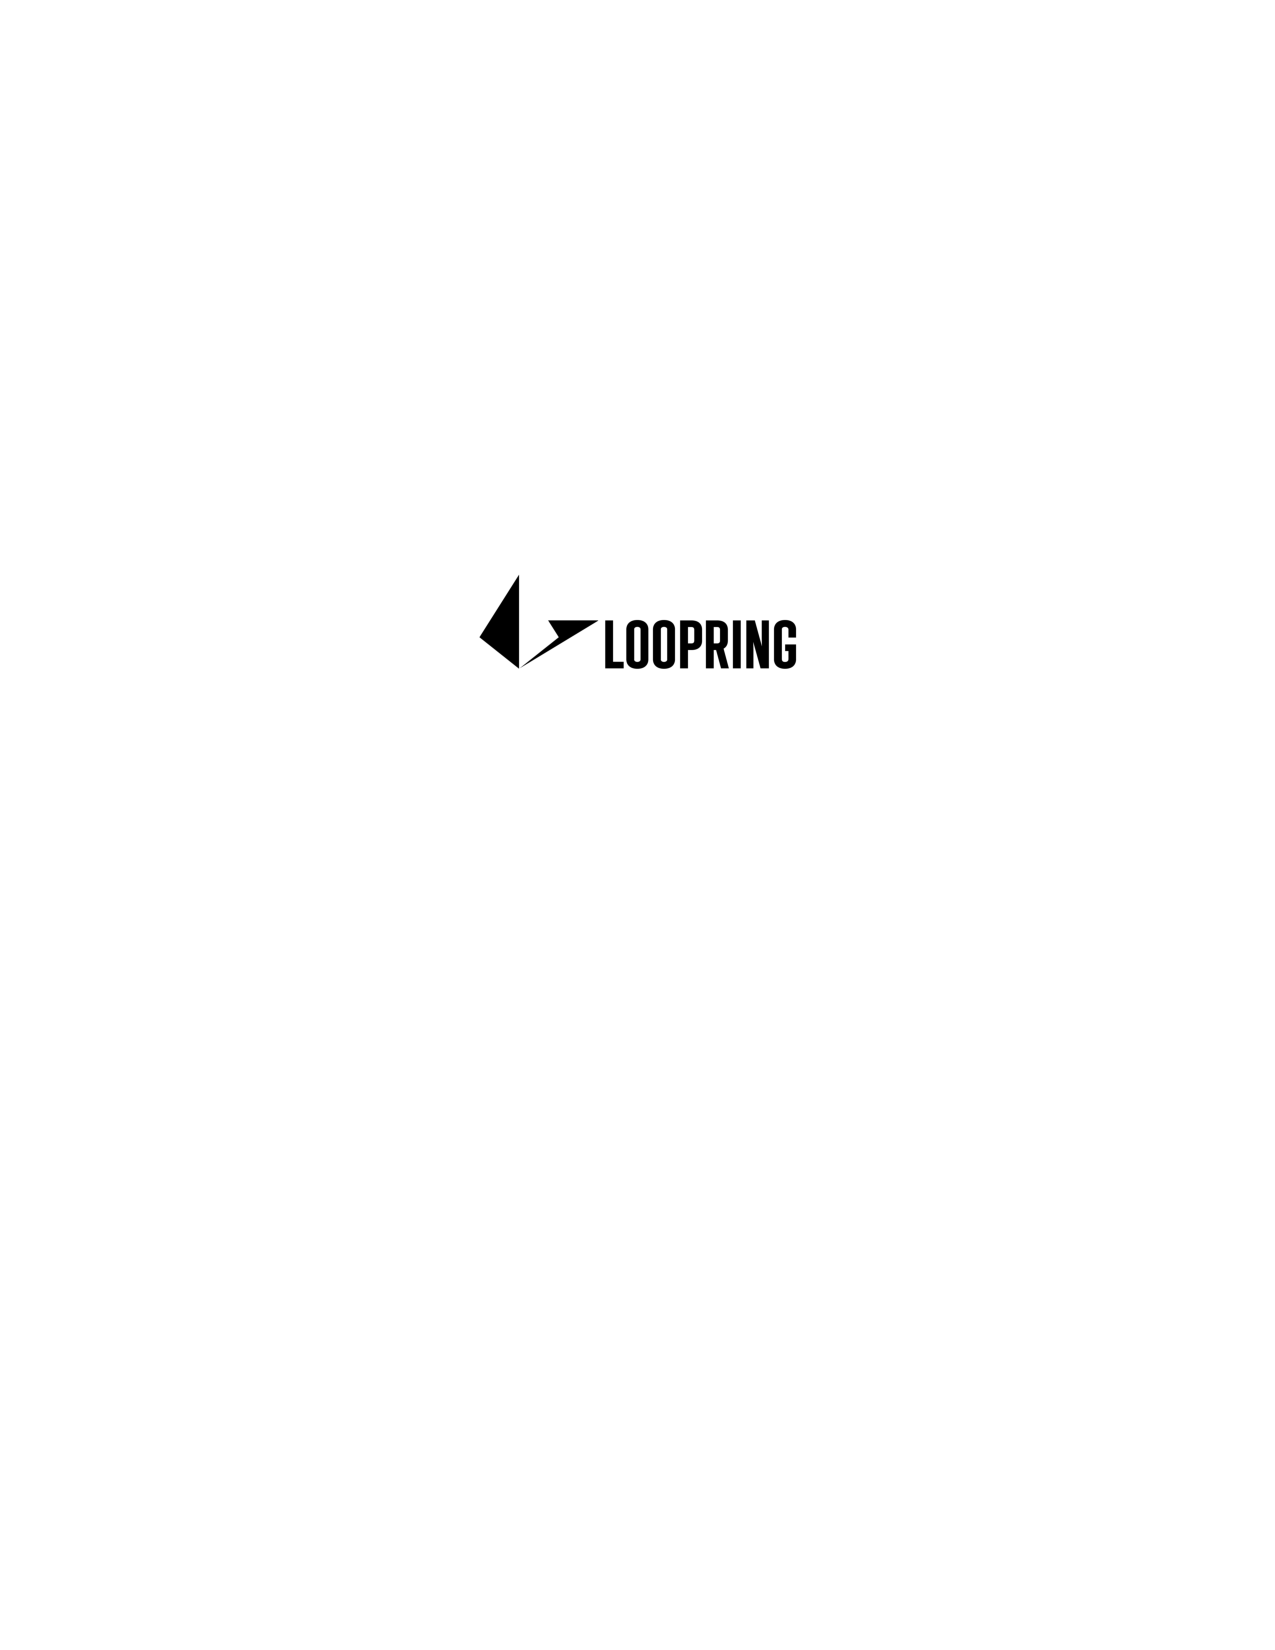
\includepdf[pages=1]{cover}
\hyphenpenalty=750

\title{\textbf{Loopring:}\\\textbf{Um Protocolo Descentralizado para Intercâmbio de Tokens}}
\author{
  Daniel Wang\\
  \texttt{daniel@loopring.org}\\
  \and
  	Jay Zhou\\
  	\texttt{jay@loopring.org}\\
  	\and
  	Alex Wang\\
  	\texttt{alex@loopring.org}\\
  	\and
  	Matthew Finestone\\
  	\texttt{matt.finestone@gmail.com}\\ 
  \\
  \texttt{https://loopring.org}
 }

\makeatletter
\def\CTEX@section@format{\Large\bfseries}
\makeatother

\makeatletter
\newenvironment{tablehere}
 {\def\@captype{table}}
 {}

\newenvironment{figurehere}
 {\def\@captype{figure}}
 {}
\makeatother
%
%\newcommand\BackgroundPic{%
%\put(0, 0){%
%\parbox[b][\paperheight]{\paperwidth}{%
%\vfill
%\centering
%\includegraphics[width=\paperwidth, height=\paperheight, %
%%keepaspectratio]{images/background.jpg}%
%]{images/background.jpg}%
%\vfill
%}}}

\begin{document}
%\AddToShipoutPicture{\BackgroundPic}
\maketitle

\begin{abstract}
Loopring é um protocolo aberto para a construção de exchanges descentralizadas. Loopring opera como um conjunto público de contratos inteligentes responsáveis por transações e liquidações, com um grupo de atores off-chain agregando e comunicando ordens. O protocolo é gratuito, extensível, e serve como um bloco de construção padronizado para aplicativos descentralizados (dApps) que incorporam funcionalidades de exchanges. Seus padrões interoperáveis facilitam, transações anônimas e livres de intermediários. Um aprimoramento importante em relação aos protocolos de exchanges descentralizadas atuais é a capacidade de fazer com que as ordens sejam embaralhadas e casadas com outras ordens dissimilares, evitando as limitações de pares de negociação de dois tokens, melhorando drasticamente a liquidez. Loopring também implementa uma solução única e robusta para impedir front-running, a injusta tentativa de enviar transações para um bloco mais rápido que o provedor de soluções original. Loopring é um blockchain agnóstico, e implementável em qualquer blockchain com funcionalidade para contratos inteligentes. No momento da escrita, é operável em Ethereum\cite{buterin2017ethereum} \cite{wood2014ethereum} e Qtum \cite{dai2017smart} com NEO \cite{atterlonn2018distributed} em construção.
\end{abstract}

\begin{multicols}{2}
\section{Introdução\label{sec:introduction}}

Com a proliferação de ativos baseados em blockchain, a necessidade de intercambiá-los entre contrapartes aumentou significativamente. À medida que milhares de novos tokens são introduzidos - incluindo a tokenização de ativos tradicionais - essa necessidade é ampliada. Seja negociando tokens por motivações de trading especulativo, ou convertendo para acessar redes por meio de seus tokens de utilidade nativos, a habilidade de intercambiar um criptoativo por outro é fundamental para o ecossistema maior. De fato, existe uma energia potencial em ativos \cite{desotocapital}, e percebendo tal energia - o desbloqueio de capital - requer não apenas posses assertivas, o que os blockchains têm invariavelmente permitido, mas a habilidade de transferir e transformar esses ativos livremente.
 
Como tal, a transação de tokens livre de intermediários (valor) é uma forma de uso atraente para a tecnologia blockchain. Até o momento, no entanto, entusiastas de cripto têm em grande parte se acomodado em negociar tokens em exchanges centralizadas tradicionais. O protocolo Loppring é necessário porque, assim como o Bitcoin \cite{nakamoto2008bitcoin} respeitosamente enfatizou que, em se tratando de dinheiro eletrônico peer-to-peer, \enquote{os principais benefícios são perdidos se um intermediário ainda é necessário para evitar gasto duplo}, da mesma forma que os benefícios dos ativos descentralizados são perdidos se eles precisarem passar por fechadas exchanges centralizadas, nas quais se depende de confiança.

Negociar tokens descentralizados em exchanges centralizadas não faz sentido de um ponto de vista filosófico, já que falham em defender as virtudes que esses projetos descentralizados abraçam. Também há numerosos riscos práticos e limitações em usar exchanges centralizadas, que estão descritos abaixo. Exchanges descentralizadas (DEXs) \cite{schuh2015bitshares} \cite{bancor} \cite{kyber} têm buscado endereçar esses problemas, e em muitos casos obtiveram sucesso em diminuir riscos de segurança através do uso de blockchains para a desintermediação. No entanto, à medida que a capacidade das DEX se torna uma infraestrutura crucial para a nova economia, há um espaço considerável para melhora da performance. Loopring busca prover ferramentas padronizadas para a dita infraestrutura com o protocolo agnóstico aberto de seu dApp.
\newpage

\section{Cenário atual das Exchanges\label{sec:current_exchange_landscape}}

\subsection{Inadequações das Exchanges Centralizadas}
Os três riscos primários das exchanges centralizadas são; 1) Falta de segurança, 2) Falta de transparência, e 3) Falta de liquidez.

\textbf{Falta de Segurança} surge de usuários tipicamente entregando o controle de suas chaves privadas (fundos) para uma entidade centralizada. Isso os expõe à possibilidade de exchanges centralizadas serem vítimas de hackers maliciosos. Os riscos de segurança e hackeamento enfrentados por todas as exchanges centralizadas são bastante conhecidos \cite{coincheckhack} \cite{mcmillan2014inside}, mas ainda são frequentemente encarados como \enquote{riscos de aposta} para negociação de tokens. Exchanges centralizadas continuam a ser um chamariz para hackers atacarem já que seus servidores custodiam acima de milhões de dólares de fundos dos usuários. Desenvolvedores de exchanges também podem cometer erros acidentais com os fundos dos usuários. Os usuários simplesmente não têm controle sob seus próprios tokens quando depositados em uma exchange centralizada.

\textbf{Falta de Transparência} expõe os usuários ao risco de exchanges desonestas agirem de forma injusta. A distinção aqui é pelas más intenções do operador da exchange, já que usuários não estão verdadeiramente negociando seus próprios ativos em exchanges centralizadas, mas sim um IOU (termo em inglês que denomina dívida, como uma nota promissória implícita). Quando tokens são enviados à wallet de uma exchange descentralizada, ela assume a custódia e oferece um IOU no lugar. Todas as negociações acontecem então, efetivamente entre os IOU's dos usuários. Para realizar saques, usuários resgatam seus IOU's com a exchange, e recebem seus tokens no endereço de suas carteiras externas. Por meio desse processo há uma falta de transparência e a exchange pode desativar ou congelar sua conta, falir, etc. Também é possível que usem ativos dos usuários para outros propósitos enquanto em custódia, como emprestá-los para terceiros. Falta de transparência pode custar aos usuários, sem necessariamente incorrer numa perda total de fundos, como no caso de taxas de transação mais altas, atrasos em picos de demanda, risco regulatório, e ordens prejudicadas por front-running.

\textbf{Falta de Liquidez.} Do ponto de vista dos operadores das exchanges, liquidez fragmentada inibe a entrada de novas exchanges por causa de dois cenários em que o vencedor leva tudo. Primeiro, a exchange com o maior número de pares de negociação ganha, porque usuários acham desejável conduzir todos as suas negociações em uma exchange. Segundo, a exchange com o maior livro de ofertas ganha, devido aos spreads de compra e venda favoráveis para cada par de negociações. Isso desencoraja a competição por novos entrantes pois é difícil para que eles construam uma liquidez inicial. Como resultado, muitas exchanges controlam uma fatia grande do mercado apesar de reclamações dos usuários e incidentes de hackeamento ainda maiores. É válido notar que à medida que exchanges centralizadas ganham fatia de mercado, se tornam um alvo de hackeamento ainda maior.

Do ponto de vista dos usuários, liquidez fragmentada reduz significativamente a experiência do usuário. Em uma exchange centralizada, usuários apenas são capazes de negociar nos pools de liquidez da própria exchange, diante de seus próprios livros de ofertas e entre seus pares de tokens disponíveis. Para intercambiar o token \verb|A| pelo token \verb|B|, usuários precisam usar uma exchange que dê suporte a ambos ou registrar em exchanges diferentes, disponibilizando informações pessoais. Usuários frequentemente precisam executar transações preliminares ou intermediárias, tipicamente entre pares de BTC ou ETH, pagando spreads de compra e venda no processo. Por fim, os livros de ordens podem não ser profundos o suficiente para completar a transação sem slippage significativa. Mesmo que a exchange pretenda processar grandes volumes, não há garantia que tais volumes e liquidez não são falsos \cite{fakevolume}.

O resultado são silos de liquidez desconectados e um ecossistema fragmentado que se assemelha ao legado do sistema financeiro, com significativo volume de negociação centralizado em poucas exchanges. As promessas de liquidez global dos blockchains não virão das exchanges centralizadas.

\subsection{Inadequações das Exchanges Descentralizadas}
Exchanges descentralizadas se diferenciam das centralizadas em parte porque os usuários têm o controle de suas chaves privadas (ativos) realizando negociações diretamente nos blockchains correspondentes. Se aproveitando da tecnologia livre de intermediários das próprias criptomoedas, elas são bem sucedidas em mitigar os riscos de segurança supracitados. No entanto, persistem os problemas no que diz respeito a performance e limitações estruturais.

A liquidez com frequência persiste como um problema já que os usuários precisam buscar contrapartes em diferentes pools e padrões de liquidez. Os efeitos da liquidez fragmentada estão presentes se as DEXs ou os dApps em geral não empregam padrões de qualidade consistentes para interoperabilidade, e se as ordens não são propagadas/compartilhadas através de uma rede extensa. A liquidez das ordens limitadas nos livros de oferta e, especificamente, sua resiliência - quão rápido as ordens consumidas são renovadas - pode afetar significativamente a otimização das estratégias de trading \cite{limitorderliquidity}. A ausência de tais padrões tem resultado não apenas em uma liquidez reduzida, mas também exposição a uma gama de contratos inteligentes proprietários potencialmente inseguros.

Além disso, já que as negociações são realizados on-chain, DEXs herdam as limitações dos blockchains correspondentes, notadamente: escalabilidade, atrasos em execuções (mineração), e modificações custosas das ordens. Portanto, livro de ofertas baseados no blockchain não escalam particularmente bem, já que executar um código no blockchain incorre em um custo (gas), tornando a cadência de múltiplos cancelamentos de ordens proibitivamente cara.

Enfim, devido ao caráter público de livros de ofertas baseados em blockchain, uma ordem enviada é visível aos mineradores enquanto espera para ser minerada no próximo bloco e posicionada no livro de ofertas. Esse atraso expõe o usuário ao risco de ser prejudicado por front-running ou por uma execução contra a sua posição.

\subsection{Soluções Híbridas}
Pelas razões acima, exchanges puramente baseadas em blockchain têm limitações que as tornam incapazes de competir com exchanges centralizadas. Existe um tradeoff entre a completa ausência de intermediários on-chain e a velocidade e flexibilidade no envio de ordens das exchanges centralizadas. Protocolos como Loopring e 0x \cite{warren20170x} mesclam a solução de liquidação on-chain com gerenciamento de ordens off-chain. Essas soluções giram em torno de contratos inteligentes abertos, mas desviam das limitações de escalabilidade através da realização de uma série de funções off-chain e dando flexibilidade aos nodes, cumprindo papéis importantes para a rede. No entanto, algumas desvantagens permanecem nos modelos híbridos também \cite{costofdecent}. O protocolo Loopring propõe diferenças significativas na nossa abordagem para uma solução híbrida ao longo deste paper.

\section{Protocolo Loopring\label{sec:loopring_protocol}}
Loopring não é uma DEX, mas um protocolo padronizado para construção de DEXs em múltiplos blockchains. Nós desmontamos as partes que compõem uma exchange tradicional e oferecemos um conjunto de contratos inteligentes públicos e atores descentralizados em seu lugar.  Os papéis na rede incluem carteiras, relays de informação, blockchains em consórcio que dividem liquidez, buscadores de livros de ofertas, mineradores de anéis e serviços de tokenização de ativos. Antes de definir cada um, nós devemos primeiro entender as ordens do Loopring.

\subsection{Anel de ordens\label{sec:order_ring}}
As ordens do Loopring são expressas no que chamamos de um Modelo Unidirecional de Ordens (UDOM)\cite{coinport2014udom}. UDOM expressa ordens como pedidos de troca de tokens, \verb|amountS|/\verb|amountB|, (quantidade de venda/compra) ao invés de melhor oferta de compra e venda. Já que toda ordem é apenas uma taxa de câmbio entre dois tokens, uma característica poderosa do protocolo é o embaralhamento e casamento de múltiplas ordens em uma negociação circular. Usando até 16 ordens ao invés de um único par de negociações, há um aumento significativo de liquidez e potencial para melhora nos preços.

\begin{center}
\begin{figurehere}
\centering
\tikzstyle{block} = [draw, fill=blue!20, rectangle, 
    minimum height=3em, minimum width=6em]
\tikzstyle{sum} = [draw, fill=blue!20, circle, node distance=1cm]
\tikzstyle{input} = [coordinate]
\tikzstyle{output} = [coordinate]
\tikzstyle{pinstyle} = [pin edge={to-,thin,black}]

\begin{tikzpicture}[
    auto, 
    node distance=2cm,
    >=latex',
    font=\bfseries\footnotesize\sffamily,
    order/.style={
		scale=0.7,
		rectangle,
		rounded corners,
		draw=black, 
		text centered,
%		text width=5cm,
		minimum height=12mm,
		fill=white
	},
	label/.style={
		scale=0.7
	}
  ]
    % We start by placing the blocks

  \node [order] (order2) 
 {%
 \begin{tabular}{l}
  \textbf{ORDEM\#2}\\
  \textbf{Proprietário: Y}\\
  \textbf{quantidadeS: 9B}\\
  \textbf{quantidadeB: 12C}
 \end{tabular}
 };
 
  \node [order, below of=order2, xshift=-3.5cm] (order1) 
 {%
 \begin{tabular}{l}
  \textbf{ORDEM\#1}\\
  \textbf{Proprietário: X}\\
  \textbf{quantidadeS: 10000A}\\
  \textbf{quantidadeB: 2B}
 \end{tabular}
 };
 
 
  \node [order, below of=order2, xshift=3.5cm] (order3) 
 {%
 \begin{tabular}{l}
  \textbf{ORDEM\#3}\\
  \textbf{Proprietário: Z}\\
  \textbf{quantidade: 100C}\\
  \textbf{quantidadeB: 160A}
 \end{tabular}
 };
 
 \draw [draw,->] (order1) -- node [label] {\textbf{7898A}} (order3);
 \draw [draw,->] (order2) -| node [label, xshift=-1.8cm] {\textbf{8B}} (order1);
 \draw [draw,->] (order3) |- node [label, xshift=1cm, yshift=0.24cm] {\textbf{98C}} (order2);
\end{tikzpicture}

\caption{Um anel de ordens de 3 ordens}
\label{fig:ring}
\end{figurehere}
\end{center}

A figura acima mostra um anel de ordens de 3 ordens. O token de venda de cada ordem (\verb|tokenS|) é também um token de compra de outra ordem (\verb|tokenB|). Isso cria um loop que permite a cada ordem intercambiar seus tokens desejados sem necessitar de uma ordem oposta para seu par. O intercâmbio em pares de transação tradicionais, é claro, ainda é executado, no que seria essencialmente um caso especial para um anel de ordens.

\begin{definition}[Anel de ordens] Se $C_{0}$, $C_{1}$, $\cdots$, $C_{n-1}$ são $n$ tokens diferentes, $O_{0\rightarrow 1}$, $\cdots$, $O_{i\rightarrow i\oplus 1}$, $\cdots$, $O_{n-1 \rightarrow 0}$ são $n$ ordens. Tais ordens podem formar um anel de ordens para negociações:
$$O_{0\rightarrow 1} \rightarrow \cdots \rightarrow O_{i\rightarrow i\oplus 1} \rightarrow \cdots \rightarrow O_{n-1\rightarrow 0} \text{, }$$
onde $n$ é o comprimento do anel de ordens, e $i\oplus 1 \equiv i+1 \mod n$.
\end{definition}

Um anel de ordens é válido quando todas as transações que o compõem podem ser executadas em uma taxa de câmbio igual ou melhor que a taxa originalmente especificada implicitamente pelo usuário. Para verificar a validade do anel de ordens, os contratos inteligentes do protocolo Loopring precisam receber anéis de ordens de mineradores de anéis onde o produto das taxas cambiais originais de todas as ordens é igual ou maior que 1.

Digamos que Alice e Bob querem intercambiar seus tokens \verb|A| e \verb|B|. Alice tem 15 tokens \verb|A| e quer 4 tokens \verb|B| por eles; Bob tem 10 tokens \verb|B| ele quer 30 tokens \verb|A| por eles.

Quem está comprando e quem está vendendo? Isso depende apenas do ativo que fixamos para dar cotações de preço. Se o token \verb|A| é a referência, então Alice está comprando o token \verb|B| pelo preço de ${15 \over 4} = 3.75$\verb|A|, enquanto Bob esta vendendo 10 tokens \verb|B| pelo preço de ${30 \over 10} = 3.00$\verb|A|. No caso de determinarmos o token \verb|B| como referência, nós dizemos que Alice está vendendo 15 tokens \verb|A| pelo preço de ${4\over 15}=0.26666667$\verb|B| e Bob está comprando 10 tokens \verb|A| pelo preço de ${10 \over 30}=0.33333334$\verb|B|. Consequentemente, quem é o comprador ou o vendedor é arbitrário.

Na primeira situação, Alice está querendo pagar um preço maior ($3.75$\verb|A|) que o preço pelo qual Bob está vendendo seus tokens, por ($3.00$\verb|A|), quando na segunda situação, Bob está querendo pagar um preço maior ($0.33333334$\verb|B|) que o preço pelo qual Alice está vendendo seus tokens ($0.26666667$\verb|B|). Está claro que a transação é possível quando quer que o comprador esteja desejando pagar um preço igual ou maior que o preço do vendedor.

\begin{equation}
{{15\over 4} \over {30\over 10}} = {{10\over 30} \over {4\over 15}}={15 \over 4} \cdot {10 \over 30} = 1.25 > 1
\end{equation}

Portanto, para que um conjunto de $n$ ordens possa ser preenchido, integral ou parcialmente, nós precisamos saber se o produto de cada uma das taxas de câmbio, como ordens de compra resultam num número maior ou igual a 1. Se sim, todas as $n$ ordens podem ser parcialmente, ou totalmente preenchidas \cite{supersymmetry}.

Se nós introduzimos uma terceira contraparte, Charlie, de modo que Alice quer dar $x_1$ tokens \verb|A| e receber $y_1$  tokens \verb|B|, Bob que dar $x_2$ tokens \verb|B| e receber $y_2$ tokens \verb|C|, e Charlie quer dar $x_3$ tokens \verb|C| e receber $y_3$ tokens \verb|A|. Os tokens necessários estão presentes, e a transação é possível se: 

\begin{equation}
{{x_1 \cdot x_2 \cdot x_3 \over y_1 \cdot y_2 \cdot y_3} \geq 1}
\end{equation}

Veja a seção \ref{anatomy} para mais detalhes sobre ordens do Loopring.

\section{Participantes do Ecossistema\label{sec:ecosystem}}
Os seguintes componentes do ecossistema, juntos, proporcionam todas as funcionalidades que uma exchange centralizada tem a oferecer.

\begin{itemize}
	\item \textbf{Wallets}: Um serviço ou interface de wallet comum que dá aos usuários acesso a seus tokens e uma forma de enviar ordens para a rede Loopring. As wallets serão incentivadas a produzir ordens através da divisão das taxas com os mineradores de anéis (veja a seção \ref{sec:token}). Acreditando que o futuro do trading se dará na segurança das wallets individuais de cada usuário, conectar esses pools de liquidez através do protocolo é primordial
	\item \textbf{Blockchain/Relay Mesh para compartilhamento de Liquidez em Consórcio}: Uma rede em malha de relays para compartilhamento de ordens e liquidez. Quando os nodes executarem o software de relays do Loopring, eles poderão se juntar a uma rede preexistente e compartilhar liquidez com outros relays através de um blockchain em consórcio. O Blockchain em consórcio que estamos construindo como primeira implementação tem compartilhamento de ordens quase instantâneo (blocos de 1 a 2 segundos) e corta parte da história antiga para permitir o download mais rápido por novos nodes. Notavelmente, relays não necessitam se juntar a esse consórcio. Eles podem atuar independentemente e não compartilhar a liquidez com outros ou podem iniciar e gerir sua própria rede de compartilhamento de liquidez.
	\item \textbf{Relays/Mineradores de Anéis}: Relays são nodes que recebem ordens das wallets ou da malha de relays, mantêm livros de ofertas públicos e histórico de negócios e, opcionalmente transmitem para outros relays (através de qualquer meio arbitrário off-chain) e/ou nodes da malha de relays. Mineração de anel é um recurso, não uma obrigação dos relays. É computacionalmente pesado e feito completamente off-chain. Nós chamamos relays com o recurso de mineração de anéis ativado, de \enquote{Mineradores de Anéis}, que produzem anéis de ordens costurando juntas, ordens que estavam separadas. Relays são livres (1) para escolherem como se comunicam uns com os outros, (2) como constroem seus livros de ofertas e, (3) como mineram anéis de ordens (algoritmos de mineração).
	\item \textbf{Contratos Inteligentes do Protocolo Loopring (LPSC)}: Uma série de contratos inteligentes públicos e gratuitos que checam os anéis de ordens recebidos de mineradores de anéis; liquidam e transferem tokens em nome dos usuários de forma livre de intermediários; incentivam mineradores de anéis e wallets com taxas; e emitem eventos. Relays/buscadores de ordens escutam a esses eventos para manter seus livros de ofertas e histórico de negócios atualizados. Veja o anexo \ref{app:protocol_ethereum} para mais detalhes.
	\item \textbf{Serviços de Tokenização de Ativos (ATS)}: Uma ponte entre ativos que não podem ser diretamente negociados no Loopring. São serviços centralizados executados por empresas e organizações de confiança. Usuários depositam ativos (reais, fiduciários ou tokens de outras redes) e têm tokens emitidos, que podem ser resgatados para depósito no futuro. Loopring não é um protocolo de exchange entre diferentes blockchains (até que surja uma solução plausível), mas ATS possibilita negociação de tokens ERC20 \cite{ERC20} em troca de ativos físicos assim como ativos de outros blockchains.
\end{itemize}

\section{Processo de Exchange\label{sec:process}}

\begin{enumerate} 
\item \textbf{Autorização no Protocolo}: Na figura \ref{fig:process}, o usuário \verb|Y| que quer fazer um trade entre tokens autoriza a LPSC a lidar com o \verb|amountS| do token \verb|B| que o usuário deseja vender. Isso não trava os tokens do usuário, que continua livre para movimentá-los enquanto a ordem é processada.

\item \textbf{Criação de Ordens}: A atual cotação e livro de ofertas do token \verb|B| vs o token \verb|C| são fornecidas por relays e outros agentes ligados à rede, como buscadores de livros de ofertas. O usuário \verb|Y| coloca uma ordem (ordem limitada) especificando a \verb|amountS| e \verb|amountB| e outros parâmetros através de qualquer interface de wallet integrada. Uma quantia de LRx pode ser adicionada à ordem como uma taxa aos mineradores de anéis; Uma taxa de LRx maior significa uma chance maior de ser processada antes pelos mineradores de anéis. O código da ordem é assinado com a chave privada do usuário \verb|Y|. 

\item \textbf{Transmissão de Ordens}: A wallet envia a ordem e sua assinatura para um ou mais relays, que atualizam seus livros de ofertas públicos. O protocolo não exige que os livros de ofertas sejam construídos de alguma maneira específica, como “primeiro-a-chegar-primeiro-a-servir”. Em vez disso, relays têm o poder de tomar suas próprias decisões de projeto em relação à construção de seus livros de oferta.

\item \textbf{Compartilhamento de Liquidez}: Relays transmitem a ordem para outros relays através de qualquer meio arbitrário de comunicação. Novamente, há flexibilidade quanto a como e se os nodes interagem. Para facilitar um certo nível de conectividade na rede, temos uma malha de relays embutida para compartilhamento de liquidez utilizando um blockchain em consórcio. Como mencionado na seção anterior, essa malha de relays é otimizada para velocidade e inclusividade. 

\begin{center}
\begin{figurehere}
\centering
\tikzstyle{block} = [draw, fill=blue!20, rectangle, 
    minimum height=3em, minimum width=6em]
\tikzstyle{sum} = [draw, fill=blue!20, circle, node distance=1cm]
\tikzstyle{input} = [coordinate]
\tikzstyle{output} = [coordinate]
\tikzstyle{pinstyle} = [pin edge={to-,thin,black}]

\begin{tikzpicture}[
    auto, 
    scale=0.7,
    node distance=2cm,
    >=latex',
    font=\bfseries\footnotesize\sffamily,
    order/.style={
		rectangle,
		scale=0.7,
		rounded corners,
		draw=black, 
		text centered,
%		text width=5cm,
		minimum height=12mm,
		minimum width=30mm,
		fill=white
	},
	role/.style={
		circle,
		scale=0.7,
		draw=black, 
		text centered,
%		text width=5cm,
		minimum height=12mm,
		minimum width=12mm,
		fill=white
	},
	steps/.style={
		circle,
		scale=0.7,
		draw=black, 
		text centered,
%		text width=5cm,
%		minimum height=12mm,
%		minimum width=12mm,
		fill=black,
		text=white
	},
	account/.style={
		circle,
		scale=0.7,
		draw=black, 
		text centered,
%		text width=5cm,
		minimum height=16mm,
		minimum width=16mm,
		fill=white
	},
	label/.style={
	  scale=0.7
    }
  ]

 
 \node [role] (user1)  {usuário X};
 \node [role, below of=user1] (user2)  {usuário Y};
 \node [role, below of=user2] (user3)  {usuário Z};
 \node [role, below of=user3, fill=gray!20] (relay1)  {relay M};
 \node [role, below of=relay1, fill=gray!20] (relay2)  {relay N};

 
 \node [order, left of=user1, xshift=-1cm] (order1) 
 {%
 \begin{tabular}{l}
  \textbf{ORDEM 1}\\
  \textbf{Proprietário: X}\\
  \textbf{quantidadeS: 10000 A}\\
  \textbf{quantidadeB: 2 B}
 \end{tabular}
 };
 
 \draw [draw, ->]  (user1) -- (order1) [label]{};
 \draw [bend right,->] (order1) to node [auto, scale=0.7] {} (relay1);
 \draw [bend right,->] (order1) to node [auto, scale=0.7] {} (relay2);
% \draw [draw, ->]  (order1) |- (relay1) [label]{};
% \draw [draw, ->]  (order1) |- (relay2) [label]{};
 
 \node [order,left of=user2, xshift=-1.5cm] (order2) 
 {%
 \begin{tabular}{l}
  \textbf{ORDEM 2}\\
  \textbf{Proprietário: Y}\\
  \textbf{quantidadeS: 9  B}\\
  \textbf{quantidadeB: 12 C}
 \end{tabular}
 };
 \draw [draw, ->]  (user2) -- (order2) [label]{};
 \draw [bend right,->] (order2) to node [auto, scale=0.7] {} (relay1);
 \draw [bend right,->] (order2) to node [auto, scale=0.7] {} (relay2);
% \draw [draw, ->]  (order2) |- (relay1) [label]{};
% \draw [draw, ->]  (order2) |- (relay2) [label]{};
% 
\node [order, left of=user3, xshift=-2cm] (order3) 
 {%
 \begin{tabular}{l}
  \textbf{ORDEM 3}\\
  \textbf{Proprietário: Z}\\
  \textbf{quantidadeS: 100 C}\\
  \textbf{quantidadeB: 160 A}
 \end{tabular}
 };
 \draw [draw, ->]  (user3) -- (order3) [label]{};
 \draw [bend right,->] (order3) to node [auto, scale=0.7] {} (relay1);
 \draw [bend right,->] (order3) to node [auto, scale=0.7] {} (relay2);
% \draw [draw, ->]  (order3) |- (relay1) [label]{};
% \draw [draw, ->]  (order3) |- (relay2) [label]{};
 
% // The Ring
\node [order, 
yshift=-1.5cm,
xshift=-2.75cm,
below of=relay2,
fill=gray!10,
minimum width=4.2cm,
minimum height=5cm] (ring) {};


\node [order, dashed, below of=relay2,yshift=-0.2cm,xshift=-2.5cm] (order11) 
 {%
 \begin{tabular}{l}
  \textbf{ORDEM 1}\\
  \textbf{Proprietário: X}\\
  \textbf{quantidadeS: 10000 A}\\
  \textbf{quantidadeB: 2 B}
 \end{tabular}
 };
 \node [order, dashed,below of=order11,xshift=-0.25cm,yshift=0.7cm] (order21) 
 {%
 \begin{tabular}{l}
  \textbf{ORDEM 2}\\
  \textbf{Proprietário: Y}\\
  \textbf{quantidadeS: 9  B}\\
  \textbf{quantidadeB: 12 C}
 \end{tabular}
 };
\node [order, dashed,below of=order21,xshift=-0.25cm,yshift=0.7cm] (order31) 
 {%
 \begin{tabular}{l}
  \textbf{ORDEM 3}\\
  \textbf{Proprietário: Z}\\
  \textbf{quantidadeS: 100 C}\\
  \textbf{quantidadeB: 160 A}
 \end{tabular}
 };
 
 % // The blockchain
\node [
rectangle,
fill=gray!20, 
right of=user1,
yshift=-4.5cm,
xshift=0.1cm,
scale=0.7,
minimum width=3.2cm,
minimum height=15.6cm] (blockchain) {\parbox[b][15cm]{1.3cm}{blockchain}};
% blockchain accounts
  \node [account, right of=user1, xshift=1cm] (account1)  {contaX};
  \node [account, right of=user2, xshift=1cm] (account2)  {contaY};
  \node [account, right of=user3, xshift=1cm] (account3)  {contaZ};
  \node [account, right of=relay1, xshift=1cm] (account4)  {contaM};
  \node [account, right of=relay2, xshift=1cm] (account5)  {contaN};
  \node [account, double, below of=account5, yshift=-1.5cm] (psc)  {LPSC};
  
 \draw [draw, ->]  (user1) -- (account1) [label]{};
 \draw [draw, ->]  (user2) -- (account2) [label]{};
 \draw [draw, ->]  (user3) -- (account3) [label]{};
% \draw [draw, ->]  (relay1) -- (account4) [label]{};
% \draw [draw, ->]  (relay2) -- (account5) [label]{};

 \draw [draw, double, thick]  (relay1) to node [auto, scale=0.5, xshift=0.15cm, yshift=0.2cm] {Compartilhamento} (relay2) [label]{};
 \draw [draw, double, thick]  (relay1) to node [auto, scale=0.5, xshift=0.15cm, yshift=-0.1cm] {de liquidez} (relay2) [label]{};

% \draw [draw, ->]  (relay1) -- (ring) [label]{};
 \draw [draw, ->]  (relay2) to node [auto, scale=0.7, xshift=-2.8cm, yshift=0.3cm] {Mineração de anéis} (ring) [label]{};
 \draw [draw, ->]  (ring) to node [auto, scale=0.7] {submitRing} (psc) [label]{};
 
 \draw [bend left,->] (account1) to node [auto, scale=0.7] {\textbf{7898 A}} (account3);
 \draw [bend left,->] (account2) to node [auto, scale=0.7] {\textbf{8 B}} (account1);
 \draw [bend left,->] (account3) to node [auto, scale=0.7] {\textbf{98 C}} (account2);
 
 \draw [bend left,->, dashed] (account1) to node [auto, scale=0.7] {} (account5);
 \draw [bend left,->, dashed] (account2) to node [auto, scale=0.7] {} (account5);
 \draw [bend left,->, dashed] (account3) to node [auto, scale=0.7, xshift=.4cm] {\textbf{Taxa}} (account5);
  
% \draw [draw,->] (order1) -- node [label] {\textbf{7898 A}} (order3);
% \draw [draw,->] (order2) -| node [label, xshift=-1.8cm] {\textbf{8 B}} (order1);
% \draw [draw,->] (order3) |- node [label, xshift=1cm, yshift=0.24cm] {\textbf{98 C}} (order2);

\node [steps, right of=user2, xshift=-0.6cm] () {1};
\node [steps, left of=user2, xshift=0.8cm] () {2};
\node [steps, left of=relay2, xshift=0.3cm, yshift=1cm] () {3};
\node [steps, left of=relay1, xshift=3.3cm, yshift=-1.6cm] () {4};
\node [steps, below of=relay2, xshift=-0.2cm, yshift=0.4cm] () {5};
\node [steps, right of=account3, xshift=-0.6cm] (step5) {6};

\draw [bend right, ->]  (psc) to node [auto, scale=0.7, xshift=0.6cm] {Liquidação} (step5) [label]{};
\end{tikzpicture}

\caption{Processo de intercâmbio do Loopring}
\label{fig:process}
\end{figurehere}
\end{center}

\item \textbf{Mineração de anéis (casamento de ordens)}: Mineradores de anéis tentam preencher a ordem integral ou parcialmente na cotação especificada ou melhor, através da combinação das mesma com múltiplas outras ordens. Mineradores de anéis são a principal razão pela qual o protocolo é capaz de fornecer alta liquidez para qualquer par. Se a cotação executada é melhor do que a que o usuário Y especificou, a margem é compartilhada entre todas as ordens no anel de ordens. Como recompensa, o minerador de anéis escolhe entre reivindicar parte dessa margem (optando pela divisão de margem e devolvendo o LRx para o usuário), ou simplesmente ficar com a taxa de LRx. 

\item \textbf{Verificação e Liquidação}: O anel de ordens é recebido pelo LPSC. Ele faz múltiplas checagens para verificar que o minerador de anéis forneceu dados e determina se o anel de ordens pode ser liquidado integralmente ou parcialmente (dependendo da taxa de câmbio das ordens no anel e tokens nas wallets dos usuários). Se todas as verificações estiverem de acordo, o contrato automaticamente transfere os tokens para os usuários e paga o minerador de anéis e a taxa da wallet ao mesmo tempo. Se o saldo do usuário \verb|Y|, como determinado pelo LPSC, é insuficiente, ele será considerado como reduzido: uma ordem reduzida irá automaticamente aumentar até seu tamanho original se forem depositados fundos suficientes em seu endereço, diferentemente de um cancelamento, que é uma operação manual de uma via única e não pode ser revertida.

\end{enumerate}

%
%\end{multicols}
%
%\begin{center}
%\begin{figurehere}
%\includegraphics[height=8cm]{images/en_protocol.png}
%\caption{Loopring Trading Process}
%\label{fig: Loopringrotocol}
%\end{figurehere}
%\end{center}
%
%\begin{multicols}{2}

\section{Flexibilidade Operacional\label{sec:business_model}}
É importante notar que o padrão aberto do Loopring permite flexibilidade significativa aos participantes, na forma como operam. Atores são livres para implementar novos modelos de negócio e gerar valor para usuários, gerando taxas de LRx em volume ou outras métricas no processo (se assim preferirem). O ecossistema é modular e feito para dar suporte à participação de uma infinidade de aplicativos.

\subsection{Livro de Ofertas\label{sec:order_book}}
Relays podem projetar seus próprios livros de ofertas da maneira que preferirem para mostrar e casar ordens dos usuários. A primeira implementação do nosso livro de ofertas segue um modelo OTC, onde ordens limitadas são posicionadas baseadas unicamente em preço. Carimbos de data e hora das ordens, em outras palavras, não têm relação com o livro de ofertas. No entanto, um relay é livre para projetar seu livro de ofertas de uma maneira tal que emule o matching engine de uma exchange centralizada, onde ordens são rankeadas por preço, respeitando também os carimbos de data e hora. Se um relay estiver inclinado a oferecer esse tipo de livro de ofertas, ele pode possuir/integrar com uma wallet, e ter tais ordens de wallet enviadas somente para o relay único, que seria então capaz de casar ordens com base no tempo. Qualquer configuração desse tipo é possível.
 
Enquanto outros protocolos DEX, às vezes exigem que os relays tenham recursos - saldo inicial de tokens para posicionar ordens compradoras - os relays do Loopring precisam apenas encontrar ordens casáveis para consumar uma negociação, e podem fazê-lo sem tokens iniciais.

\subsection{Compartilhamento de Liquidez\label{sec:liquidity_sharing}}
Relays são livres para projetar como compartilham liquidez (ordens) entre si. Nosso blockchain em consórcio é apenas uma solução para se conseguir isso, e o ecossistema é livre para se conectar e comunicar da maneira que bem preferir. Além de se juntar a um blockchain em consórcio, eles podem construir e gerenciar seus próprios blockchains, criando regras/incentivos como preferirem. Relays podem também trabalhar sozinhos, como visto na implementação de wallet sensível ao tempo. É evidente que há claras vantagens em comunicar com outros relays em busca de efeitos de rede, no entanto, diferentes modelos de negócios podem necessitar projetos de compartilhamento específicos e dividir taxas de múltiplas maneiras.

\section{Especificações do Protocolo\label{sec:protocol}}

\subsection{Anatomia de uma Ordem\label{anatomy}}
Uma ordem é um pacote de dados que descreve a intenção de negociação do usuário. Uma ordem Loopring é definida usando o Modelo Unidirecional de Ordens, ou UDOM, como abaixo:

\begin{verbatim}
  message Order {
    address protocol;
    address owner;
    address tokenS;
    address tokenB;
    uint256 amountS;
    uint256 amountB;
    unit256 lrcFee
    unit256 validSince; // Seconds since epoch
    unit256 validUntil; // Seconds since epoch
    uint8   marginSplitPercentage;  // [1-100]
    bool    buyNoMoreThanAmountB;
    uint256 walletId;
    // Dual-Authoring address
    address authAddr;
   // v, r, s are parts of the signature
    uint8   v;       
    bytes32 r;
    bytes32 s;
    // Dual-Authoring private-key,
    // not used for calculating order's hash,
    // thus it is NOT signed.
    string  authKey;          
    uint256 nonce;
  }
\end{verbatim}

Para certificar a origem de uma ordem, ela é assinada diante do código de seus parâmetros, excluindo \verb|authAddr|, com a chave privada do usuário. O parâmetro \verb|authAddr| é usado para assinar anéis de ordens dos quais esta ordem faz parte, o que impede o front-running. Por favor consulte a seção \ref{sec:dual_authoring} para mais detalhes. A assinatura é representada pelos campos \verb|v|, \verb|r|, e \verb|s|, e é enviada juntamente com os parâmetros da ordem através da rede. Isso garante que a ordem permanecerá imutável durante todo o seu tempo de vida. Mesmo que a ordem nunca mude, o protocolo ainda pode computar seu estado atual baseado no balanço de seu endereço juntamente com outras variáveis.

O UDOM não inclui um preço (o que precisa ser um número em ponto flutuante por natureza), mas, em vez disso, usa o termo \verb|taxa|, ou $r$, que é expresso como \verb|amountS|/\verb|amountB|. A taxa não é um número em ponto flutuante mas uma expressão que será avaliada apenas com outros números inteiros não assinados sob demanda, para manter todos os resultados intermediários como números inteiros não assinados e aumentar a precisão de cálculo.

\subsubsection{Montantes de Compra}

Quando um minerador de anéis casa ordens através do anel, é possível que uma taxa melhor seja executável, permitindo que usuários fiquem com mais \verb|tokenB| do que \verb|amountB| especificados. no entanto, se \verb|buyNoMoreThanAmountB| é definido como \verb|True|, o protocolo assegura que usuários recebam não mais que \verb|amountB| do \verb|tokenB|. Portanto, o parâmetro \verb|buyNoMoreThantokenB| do UDOM, determina quando uma ordem é considerada completamente preenchida. \verb|buyNoMoreThantokenB| aplica um teto em ambos \verb|amountS| ou \verb|amountB|, e permite que usuários expressem intenções de negociação mais granulares do que ordens de compra/venda tradicionais.

Por exemplo: com \verb|amountS| = 10 e \verb|amountB| = 2, a taxa $r$ = 10/2 = 5. Portanto o usuário está querendo vender 5 \verb|tokenS| para cada \verb|tokenB|. O minerador de anéis casa e dá ao usuário a taxa de 4, permitindo que ele receba 2.5 \verb|tokenB| ao invés de 2. No entanto, se o usuário quer apenas 2 \verb|tokenB| e definiu a bandeira do \verb|buyNoMoreThanAmountB| para \verb|True|, o LPSC executa a transação a uma taxa de of 4 e o usuário vende 4 \verb|tokenS| para cada \verb|tokenB|, efetivamente economizando 2 \verb|tokenS|. Tenha em mente que isso não leva em conta taxas de mineração (Veja seção \ref{sec:fee_model}).

De fato, se usarmos
\begin{verbatim}
	      Order(amountS,tokenS,
	            amountB,tokenB,
	            buyNoMoreThantokenB)
\end{verbatim}
para representar uma ordem de uma forma simplificada, então para mercados de ETH/USD em uma exchange tradicional, o modelo tradicional de compra e venda pode expressar a 1ª e a 3ª ordem abaixo, mas não as outras duas:

\begin{enumerate}
	\item Vender 10 ETH ao preço de 300 USD/ETH. Ordem expressa como: \verb|Order(10, ETH, 3000, USD, False)|.
	\item Vender ETH ao preço de 300 USD/ETH para obter 3000 USD. Ordem expressa como: \verb|Order(10, ETH, 3000, USD, True)|.
	\item Comprar 10 ETH ao preço de 300 USD/ETH, ordem expressa como: \verb|Order(3000, USD, 10, ETH, True)|.
	\item Gastar 3000 USD para comprar o maior número possível de ETH pelo preço de 300 USD/ETH. Ordem expressa como: \verb|Order(3000, USD, 10, ETH, False)|.
\end{enumerate}

\subsection{Verificação de Anéis\label{sec:ring_verification}}
Os contratos inteligentes do Loopring não calculam taxas de câmbio ou quantidade, mas precisam receber e verificar o que os mineradores de anéis fornecem para esses valores. Tais cálculos são feitos através de mineradores de anéis por duas razões principais: (1) linguagens de programação para contratos inteligentes, como a solidity\cite{dannen2017introducing} no Ethereum, não têm suporte para matemática de ponto flutuante, especialmente $pow(x, 1/n)$ (calculando a n-ésima raiz de um número em ponto flutuante), e (2) é desejável que a computação seja feita off-chain para reduzir computação do blockchain e o custo.

\subsubsection{Verificação de Sub Anel\label{sec:sub_ring_check}}
Este passo impede que arbitradores realizem injustamente toda a margem em um anel de ordens por implementar novas ordens nele. Essencialmente, uma vez que um anel de ordens válido é encontrado por um minerador de anéis, poderia ser tentador adicionar outras ordens ao anel de ordens para absorver completamente a margem dos usuários (descontos de taxa). Como ilustrado pela figura \ref{fig:subring} abaixo, calculando cuidadosamente $x1$, $y1$, $x2$ e $y2$ você fará o produto de todas as taxas das ordens ser exatamente 1 então não haverá desconto de taxa.

\begin{center}
\begin{figurehere}
\centering
\tikzstyle{block} = [draw, fill=blue!20, rectangle, 
    minimum height=3em, minimum width=6em]
\tikzstyle{sum} = [draw, fill=blue!20, circle, node distance=1cm]
\tikzstyle{input} = [coordinate]
\tikzstyle{output} = [coordinate]
\tikzstyle{pinstyle} = [pin edge={to-,thin,black}]

\begin{tikzpicture}[
    auto, 
    node distance=2cm,
    >=latex',
    font=\bfseries\footnotesize\sffamily,
    order/.style={
		scale=0.7,
		rectangle,
		rounded corners,
		draw=black, 
		text centered,
%		text width=5cm,
		minimum height=12mm,
		fill=white
	},
	label/.style={
		scale=0.7
	}
  ]
    % We start by placing the blocks

  \node [order] (order2) 
 {%
 \begin{tabular}{l}
  \textbf{ORDEM 2}\\
  \textbf{Proprietário: Y}\\
  \textbf{quantidadeS: 9B}\\
  \textbf{quantidadeB: 12C}
 \end{tabular}
 };
 
  \node [order, below of=order2, xshift=-3.5cm] (order1) 
 {%
 \begin{tabular}{l}
  \textbf{ORDEM 1}\\
  \textbf{Proprietário: X}\\
  \textbf{quantidadeS: 10000 A}\\
  \textbf{quantidadeB: 2 B}
 \end{tabular}
 };
 
 
  \node [order, below of=order2, xshift=3.5cm] (order3) 
 {%
 \begin{tabular}{l}
  \textbf{ORDEM 3}\\
  \textbf{Proprietário: Z}\\
  \textbf{quantidadeS: 100 C}\\
  \textbf{quantidadeB: 160 A}
 \end{tabular}
 };
 
   \node [order, below of=order3, fill=gray!20] (order4) 
 {%
 \begin{tabular}{l}
  \textbf{ORDEM 4}\\
  \textbf{Proprietário: M}\\
  \textbf{quantidadeS: x1 A}\\
  \textbf{quantidadeB: y1 B}
 \end{tabular}
 };
 
 
  \node [order, below of=order1, fill=gray!20] (order5) 
 {%
 \begin{tabular}{l}
  \textbf{ORDEM 5}\\
  \textbf{Proprietário: addressM}\\
  \textbf{quantidadeS: x2 C}\\
  \textbf{quantidadeB: y2 A}
 \end{tabular}
 };
 
 \draw [draw,->] (order1) -- node [label, xshift=-2cm] {} (order5);
 \draw [draw,->] (order2) -| node [label, xshift=-1.6cm] {} (order1);
 \draw [draw,->] (order3) |- node [label, xshift=1cm] {} (order2);
 \draw [draw,->] (order4) -- node [label, xshift=1.8cm] {} (order3);
 \draw [draw,->] (order5) -- node [label, yshift=0.2cm] {} (order4);
  
\end{tikzpicture}

\caption{Um anel de ordens com sub anel}
\label{fig:subring}
\end{figurehere}
\end{center}

Isso apresenta zero risco e zero valor acrescentados à rede, e é considerado conduta desleal pelo minerador de anéis. Para impedir isso, Loopring precisa que um loop válido não possa conter nenhum sub anel. Para verificar isso, o LPSC se certifica que um token não possa estar em uma posição de compra ou venda duas vezes. No diagrama acima, nós podemos ver que token \verb|A| é um token de venda duas vezes e um token de compra duas vezes, o que não seria permitido.

\subsubsection{Verificação da Taxa de Câmbio\label{sec:fill_rate_check}}

Os cálculos de taxa de câmbio no anel de ordens são feitos por mineradores de anéis pelas razões expostas acima. É o LPSC que precisa se certificar que eles estejam corretos.  Primeiro  ele verifica que a taxa de compra que o minerador de anéis pode executar para cada ordem é igual ou menor que a taxa de compra original definida pelo usuário. Isso garante que os usuários tenham pelo menos a taxa de câmbio pela qual pediram ou melhor na transação. Uma vez que as taxas de câmbio são confirmadas, o LPSC se assegura que cada ordem no anel de ordens  compartilha o mesmo desconto na taxa. Por exemplo, se a taxa descontada é $\gamma$, então o preço para cada ordem será:

$r_{0\rightarrow 1} \cdot (1-\gamma)$, $r_{1\rightarrow 2} \cdot (1-\gamma)$, $r_{2 \rightarrow 0} \cdot (1-\gamma)$, e satisfará:
\begin{equation}
r_{0\rightarrow 1} \cdot (1-\gamma)\cdot r_{1\rightarrow 2} \cdot (1-\gamma) \cdot r_{2 \rightarrow 0} \cdot (1-\gamma) = 1
\end{equation}
consequentemente: 
\begin{equation}
\gamma = 1- \frac{1}{\sqrt[3]{r_{0\rightarrow 1} \cdot r_{1\rightarrow 2} \cdot r_{2\rightarrow 0}}}\text{.}
\end{equation}
Se a transação cruza $n$  ordens, o \texttt{discount} é: 
\begin{equation}
\gamma = 1- \frac{1}{\sqrt[n]{\prod_{i=0}^{n-1} r^i}} \text{,}
\end{equation}

onde $r^i$  é a taxa de rotatividade da $i$-ésima ordem. Obviamente, apenas quando a taxa de desconto é $\gamma \ge 0$, tais ordens podem ser preenchidas; e a real taxa de câmbio da ordem i-ésima ($O^i$) é $\hat{r^i} = r^i \cdot (1-\gamma)$, $\hat{r^i}\le r^i$.

Relembre nosso exemplo anterior, onde Alice tem 15 tokens \verb|A| e quer 4 tokens \verb|B| por eles, Bob tem 10 tokens \verb|B| e quer 30 tokens \verb|A| por eles. Se o token \verb|A| é a referência, então Alice está comprando tokens \verb|B| por $\frac{15}{4}$ = 3.75\verb|A|, enquanto Bob está vendendo tokens \verb|B| por $\frac{30}{10}$ = 3.00\verb|A|. Para calcular o desconto: $\frac{150}{120}$ = 1.25 então $\frac{1}{1.25}$ = 0.8 = $(1 −- \gamma)^2$. Portanto, a taxa de câmbio que processa a transação equitativa para ambas as partes é $\sqrt{0.8}$ $\cdot$ 3.75 $\approx$ 3.3541 tokens \verb|A| por tokens \verb|B|.

Bob dá 4 tokens \verb|B| e recebe 13.4164 tokens \verb|A|, que é mais do que os 12 que ele esperava pelos 4 tokens. Alice recebe 4 tokens \verb|B| como pretendia, mas dá apenas 13.4164 tokens \verb|A| em troca, que é menos do que os 15 que ela pretendia dar pelos 4 tokens.
Note que, uma porção dessa margem será destinada a pagar taxas para incentivar mineradores (e wallets). (Veja seção \ref{sec:fee_model}).

\subsubsection{Acompanhamento de transações \& Cancelamento}
Um usuário pode cancelar parcialmente ou integralmente uma ordem pelo envio de uma transação especial para o LPSC, contendo os detalhes sobre a ordem e as quantidades para cancelar. O LPSC leva isso em conta, armazena as quantidades para cancelar e emite um evento \verb|OrderCancelled| para a rede. O LPSC mantém o controle de montantes preenchidos ou cancelados armazenando seus valores usando o código da ordem como um identificador. Estes dados são publicamente acessíveis, e eventos de \verb|OrderCancelled| / \verb|OrderFilled| são emitidos quando eles mudam. Rastrear esses eventos é fundamental para o LPSC durante a etapa de liquidação do anel de ordens.

LPSC também suporta o cancelamento de todas as ordens para qualquer par de negociação com o evento \verb|OrdersCancelled| e cancelamento de todas as ordens para um endereço com o evento \verb|AllOrdersCancelled|.

\subsubsection{Escalabilidade de Ordens\label{sec:order_scaling}}
Ordens são escaladas de acordo com com o histórico de quantidades preenchidas e canceladas, e o saldo corrente das contas dos emissores. O processo encontra a ordem com o  menor montante a ser preenchido de acordo com as características acima e as usa como referência  para escalar todas as transações no anel de orens.

O encontro da ordem de menor valor pode ajudar a descobrir o volume de preenchimento para cada ordem. Por exemplo, se a ordem $i$-ésima é a ordem de menor valor, o número de tokens vendidos por cada ordem $\hat{s}$ e o número de tokens adquiridos $\hat{b}$ por cada ordem pode ser calculado como:

\[
\begin{split}
&\hat{s}^{i}=\overline{s}_i\text{, } \hat{b}^{i}=\hat{s}^{i}/ \hat{r}^i\text{, }\text{;}\\
&\hat{s}^{i\oplus 1}=\hat{b}^i\text{, } \hat{b}^{i\oplus 1}=\hat{s}^{i\oplus 1}/ \hat{r}^{i\oplus 1}\text{;}\\
&\hat{s}^{i\oplus 2}=\hat{b}^{i\oplus 1}\text{, } \hat{b}^{i\oplus 2}=\hat{s}^{i\oplus 2}/ \hat{r}^{i\oplus 2}\text{;}\\
& ...
%\text{.}
\end{split}
\]
onde $\overline{s}_i$ é o saldo restante após as ordens serem preenchidas parcialmente.

Durante a implementação, nós podemos seguramente assumir que qualquer ordem no anel de ordens tenha o menor valor, e então iterar pelo anel de ordens no máximo duas vezes para calcular o volume de preenchimento de cada ordem.

Exemplo: Se a menor quantidade a ser preenchida comparada com a ordem original é 5\%, todas as transações no anel de ordens são reduzidas para 5\%. Uma vez que as transações são completadas, a ordem que havia sido considerada como de menor quantidade restante a ser preenchida deverá ser completamente preenchida.

\subsection{Liquidação de Anéis\label{sec:settlement}}
Se o anel de ordens preenche todos os requisitos anteriores, ele pode ser fechado e as transações podem ser efetuadas. Isso significa que todas as $n$ ordens formam um anel de ordens fechado, conectado como na figura 4:

\begin{center}
\begin{figurehere}
\centering
\begin{tikzpicture}[
circle/.style={
		scale=0.75,
		rounded corners,
		draw=black, 
		text centered,
		}
]

\def \n {6}
\def \m {4}
\def \radius {1.1cm}
\def \margin {12} % margin in angles, depends on the radius

\foreach \s in {1,...,\m}
{
  \node[draw, circle] at ({360/\n * (\s - 1)}:\radius) {$O^\s$};
  \draw[<-, >=latex] ({360/\n * (\s - 1)+\margin}:\radius) 
    arc ({360/\n * (\s - 1)+\margin}:{360/\n * (\s)-\margin}:\radius);
}

\node[draw, circle] at ({360/\n * 4}:\radius) {$O^5$};
  \draw[<-, dashed, >=latex] ({360/\n * 4+\margin}:\radius) 
    arc ({360/\n * 4+\margin}:{360/\n * (5)-\margin}:\radius);
    
\node[draw, circle] at ({360/\n * 5}:\radius) {$O^n$};
  \draw[<-, >=latex] ({360/\n * 5+\margin}:\radius) 
    arc ({360/\n * 5+\margin}:{360/\n * (6)-\margin}:\radius);
\end{tikzpicture}
\caption{Liquidação do anel}
\label{fig:settlement}
\end{figurehere}
\end{center}

Para fazer as transações, o LPSC usa o contrato inteligente \verb|TokenTransferDelegate|. A introdução de tal delegado torna a melhoria do protocolo do contrato inteligente mais fácil, já que todas as ordens apenas precisam autorizar esse delegado ao invés de versões diferentes do protocolo.

Para cada ordem no anel de ordens, um pagamento de \verb|tokenS| é feito para a próxima ordem ou a anterior dependendo da implementação. Em seguida, a taxa do minerador de anéis é paga dependendo do modelo de taxa escolhido por ele. Finalmente, uma vez que todas as transações são efetuadas, um evento \verb|RingMined| é emitido.

\subsubsection{Eventos emitidos\label{sec:events}}
O protocolo emite eventos que permitem que relays, buscadores de ordens, e outros atores recebam atualizações do livro de ofertas da maneira mais eficiente possível. Os eventos emitidos são:

\begin{itemize}
	\item \textbf{OrderCancelled}: Uma ordem específica foi cancelada.
	\item \textbf{OrdersCancelled}: Todas as ordens de um par de negociações de um endereço de posse foram canceladas.
	\item \textbf{AllOrdersCancelled}: Todas as ordens de todos os pares de negociação  de um endereço de posse foram canceladas.
	\item \textbf{RingMined}: Um anel de ordens foi liquidado com sucesso. Esse evento contém dados relacionados a cada transferência de tokens em anel interno.
\end{itemize}

\section{Token LRx\label{sec:token}}
LRx é a nossa notação generalizada de tokens. LRC é o token do Loopring na Ethereum, LRQ na Qtum, e LRN na NEO, etc. Outros tipos de LRx serão introduzidos no futuro à medida que o Loopring é implantado em outros blockchains públicos.

\subsection{Modelo de Taxas\label{sec:fee_model}}
Quando um usuário cria uma ordem, ele especifica um montante de LRx a ser pago para o minerador de anéis como uma taxa, em conjunto com a porcentagem da margem (\verb|marginSplitPercentage|) feito na ordem em que o minerador de anéis possa reivindicar. Isso é chamado de Divisão de Margem (Margin Split). A decisão sobre qual escolha fazer (taxa ou divisão de margem) é deixada ao minerador de anéis.
\newpage
 
A representação da divisão de margem:
\begin{center}
\begin{figurehere}
\centering
\begin{tikzpicture}[
scale=1,
font=\bfseries\footnotesize\sffamily,
classical/.style={thick,<->,shorten >=2pt,shorten <=2pt,>=stealth},
oneway/.style={->,dashed,shorten >=2pt,shorten <=2pt,>=stealth}
]
    % Draw axes
    \draw [->,thick] (0,1) node (yaxis) [above] {$$}
        |- (6.2,0) node (xaxis) [right] {$$};
        
    \draw
  	(4,0) coordinate (A)
  	(4,1) coordinate (A2)
  	(4.8,-0.6) coordinate (B)
  	(4.8,1) coordinate (B2)
  	(6,-0.6) coordinate (C)
  	(6,1) coordinate (C2);
  	
  	\fill [draw=none, fill=gray!20] 
    (4.8, 0) rectangle (6, 1);
    
  	\fill [draw=none, fill=gray!10] 
    (0, -0.6) rectangle (4.8, 0);
	\draw[thick] (0, -0.6) -- (0, 0.6) node[below]{$$};
  	\draw[thick, thin] (A) -- (A2) node[below]{$$};
  	\draw[thick, thin] (B) -- (B2) node[below]{$$};
  	\draw[thick] (C) node[below, xshift=0.5cm]{$Total Buy Amount$} -- (C2) ;
  	
  	\draw[classical] (0, 0.5) -> (4, 0.5) node[below]{$$};
  	\draw[classical] (4, 0.75) -> (4.8, 0.75) node[below]{$$};
%  	\draw[classical] (4.8, 0.5) -> (6, 0.5) node[below]{$$};
  	\draw[classical] (4, 0.25) -> (6, 0.25) node[below]{$$};
  	
  	\draw[oneway] (2, 1.2) node[above]{$Order Original Buy Amount$} -- (2, 0.5);
  	\draw[oneway] (4.4, 2.2) node[above]{$Additional Buy Amount$} -- (4.4, 0.75);
  	\draw[oneway] (5.4, 1.6) node[above]{$Margin Split$} -- (5.4, 1);
  	\draw[oneway] (5, -1.2) node[below]{$Margin$} -- (5, 0.25);
  	\draw[oneway] (2.4, -1.2) node[below]{$Order Actual Buy Amount$} -- (2.4, -0.5);
\end{tikzpicture}
\caption{Uma divisão de margem de 60\%}
\label{fig:marginsplit}
\end{figurehere}
\end{center}

Se a margem no minerador de anéis é pequena demais, ele irá escolher a taxa de LRx. Se, ao contrário, a margem é grande o suficiente para que a divisão de margem resultante valha muito mais que a taxa de LRx, ele irá escolher a divisão de margem. Há outra condição, no entanto: quando o minerador de anéis escolhe a divisão de margem, ele precisa pagar ao usuário (criador da ordem) uma taxa, que é igual ao LRx que o usuário teria pago ao minerador de anéis como taxa. Isso aumenta o limite de onde o minerador de anéis irá escolher a divisão de margem. Isso permite que os mineradores de anéis recebam uma renda constante em anéis de ordem de baixa margem em compensação por receber menos renda em anéis de ordens de margens mais altas. Nosso modelo de taxas é baseado na expectativa que à medida que o mercado cresce e amadurece, haverão menos anéis de ordens de margens altas, assim necessitando taxas fixas de LRx como incentivo.
Nós terminamos com o seguinte gráfico:

\begin{center}
\begin{figurehere}
\centering
\begin{tikzpicture}[
font=\bfseries\footnotesize\sffamily,
oneway/.style={->,dashed,shorten >=2pt,shorten <=2pt,>=stealth},
scale=1]
    % Draw axes
    \draw [<->,thick] (0,2.7) node (yaxis) [above] {$y$}
        |- (5,0) node (xaxis) [right] {$x$};
        
    \draw
  	(1,1) coordinate (A)
  	(2,1) coordinate (B);
  	  	
  	\draw[thick] (B) -- (3.7,2.7);
  	\draw[dotted] (B) -- (2,0) node[below] {$2f$};
  	\draw[dotted] (A) -- (1,0) node[below] {$f$};
  	\draw[thick,color=gray!70] (0,0) -- (2.7,2.7);
  	\draw[thick] (0,1) node[left] {$f$}--(B) node[     ]{$$};
 	\draw[oneway] (4,1) node[right]{$Expected Mining Income$} -- (3, 2);
\end{tikzpicture}
\caption{Modelo de Taxas do Loopring}
\label{fig:feemodel}
\end{figurehere}
\end{center}

onde $f$ é a taxa do LRx, $x$ é a divisão de margem, $y$ é o pagamento da mineração. $y=max(f, x-f)$ como indicado pela linha sólida; se a taxa do LRx para a ordem é $0$, a equação é $y=max(0, x - 0)$ o que se simplifica para $y=x$ como indicado pela linha cinza. As consequências são:

\begin{enumerate}
\item Se a margem dividida é 0, os mineradores de anéis escolherão a taxa fixa do LRx e ainda serão incentivados.
\item Se a taxa do  LRx é 0, é gerada a linha cinza  e o pagamento será baseados em um modelo geral linear.
\item Quando o rendimento de margem dividida  é maior que  2x (taxa de LRx), mineradores de anéis escolhem a divisão de margem e pagam LRx ao usuário.
\end{enumerate}

É importante notar que, se a taxa de LRx é diferente de zero, independentemente da opção que o minerador de anéis escolhe, haverá sempre um transferência de LRx entre ele e o emissor da ordem. Ou o minerador de anéis ganha a taxa do LRx, ou paga a taxa do LRx de volta para o emissor para ficar com a margem dividida.

Mineradores de anéis vão compartilhar uma certa porcentagem de taxas com wallets. Quando um usuário envia uma ordem através de uma wallet e ela é preenchida, a wallet é recompensada com uma porção das taxas ou margem dividida. Ainda que isso seja modular, e modelos de negócios únicos e implementações sejam possíveis, nossa inclinação é que as wallets recebam aproximadamente 20\%-25\% das taxas geradas. Wallets representam um alvo primário para a integração do protocolo Loopring já que têm a base de usuários, mas pouca ou nenhuma fonte de rendimentos.

\subsection{Governança Descentralizada}
Como sua essência, o protocolo Loopring é um protocolo social no sentido de depender da coordenação entre membros para operar de maneira efetiva em direção a um objetivo. Isso não é diferente da maioria dos protocolos criptoeconômicos e, de fato, sua utilidade é largamente protegida pelos mesmos mecanismos de problemas de coordenação \cite{vitalikgovernance}, equilíbrio implacável de gatilhos, e racionalidade limitada. Para este fim, tokens LRx não são apenas usados para pagar taxas, mas também para alinhar os incentivos financeiros dos vários participantes da rede. Tal alinhamento é necessário para a adoção mais ampla de qualquer protocolo, mas é particularmente importante para protocolos de exchanges, dado que o sucesso se apoia fortemente em melhorar liquidez em um ecossistema robusto e descentralizado.

Tokens LRx serão usados para efetuar atualizações de protocolo através de governança descentralizada. Atualizações de contratos inteligentes serão governadas por detentores de tokens para garantir continuidade e segurança, e para atenuar os riscos de ter a liquidez sugada por incompatibilidade. Dado que contratos inteligentes não podem ser alterados após serem implantados, há um risco de que os dApps ou usuários finais continuem a interagir com versões descontinuadas e fiquem sem acesso a contratos atualizados. A capacidade de atualização é crucial para o sucesso do protocolo já que ele precisa se adaptar às demandas do mercado e aos blockchains subjacentes. A governança descentralizada pelas partes interessadas no LRx vai permitir atualizações nos protocolos dos contratos inteligentes sem interromper dApps ou usuários finais, ou depender demasiadamente da abstração dos contratos inteligentes. Os tokens LRx têm um fornecimento fixo e, no caso do LRC, uma porcentagem fica congelada na Fundação Loopring e alocados em fundos destinados à comunidade \cite{LRCtokendoc}.

No entanto, os proprietários de tokens LRx não são as únicas partes interessadas a serem consideradas na orientação do protocolo: relays/mineradores de anéis, wallets, desenvolvedores e outros, são parte integrante do ecossistema e sua voz deve ser ouvida. De fato, dado que esses agentes não precisam deter nenhum token LRx para desempenhar seus respectivos papéis (já que market makers/takers tradicionais são inexistentes, as reservas iniciais de tokens não são obrigatórias) devemos permitir métodos alternativos para que seus interesses sejam respeitados. Além disso, a votação \enquote{simples} baseada em tokens, tanto on-chain e off-chain é uma remediação imperfeita para o desacordo, já que a baixa presença de eleitores e a concentração da posse de tokens representam riscos. Assim, o objetivo é implementar um modelo de governança que é construído em camadas e se apoia no entendimento compartilhado de que alguns conjuntos de processos de tomada de decisão são a norma. Isso pode ser facilitado através de instituições de coordenação que trazem sinalizações de uma diversidade de participantes e, talvez, de pontos focais preestabelecidos do protocolo. À medida que isso se realiza, a Fundação Loopring irá inevitavelmente evoluir de desenvolvedores de protocolo para administradores de protocolo.

\section{Fraude e Proteção Contra Ataques}

\subsection{Prevenção de Front-Running\label{sec:dual_authoring}}
Em exchanges descentralizadas, front-running é quando alguém tenta copiar a solução de trade de outro node, e a tem minerada antes da transação original que está no pool de transações pendentes (mempool). Isso pode ser alcançado definindo uma taxa de transação mais alta (gas price). O esquema principal do front-running no Loopring (e qualquer protocolo para casamento de ordens) é o furto de ordens: quando um front runner rouba uma ou mais ordens de uma transação com liquidação pendente no anel de ordens; e, especifico ao Loopring: quando um front runner rouba todo o anel de ordens por uma transação pendente.

Quando uma transação submitRing não é confirmada e ainda está no pool de transações pendentes, qualquer um pode facilmente percebe-la e substituir o \verb|minerAddress| pelo seu próprio endereço (o \verb|filcherAddress|), e então eles podem re-assinar o payload com \verb|filcherAddress| para substituir a assinatura do anel de ordens. O filcher pode definir um preço de gas mais alto e enviar uma nova transação esperando que os mineradores de blocos a selecionem no próximo bloco ao invés da transação submitRing original.

Soluções prévias para este problema tiveram lados negativos relevantes: requerendo mais transações e portanto, custando mais gas aos mineradores de anéis; e precisando de pelo menos o dobro de blocos para liquidar o anel de ordens. Nossa nova solução, Dual Authoring \cite{dualauthor}, envolve o mecanismo de definir até dois níveis de autorização para ordens - um para liquidação, e outro para mineração de anéis.
\newline

Processo Dual Authoring:

\begin{enumerate}
\item Para cada ordem, o software da wallet irá gerar um par de chave pública/chave privada aleatório, e colocá-lo no snippet JSON da ordem. (Uma alternativa é usar o endereço derivado da chave pública ao invés da chave pública em si para reduzir o tamanho de bytes. Nós usamos \verb|authAdd| para representar tal endereço, e \verb|authKey| para representar a chave privada correspondente ao \verb|authAddr|).
\item Computar o código da ordem com todos os campos na ordem, (exceto \verb|r|, \verb|v|, \verb|s|, e \verb|authKey|), e assinar o código usando a chave privada do \verb|proprietário| (não \verb|authKey|).
\item A carteira irá enviar a ordem juntamente com o \verb|authKey| para os relays para a mineração de anéis. Mineradores de anéis verificarão que o \verb|authKey| e o \verb|authAddr| estão corretamente casados e a assinatura da ordem é válida no que se refere ao endereço do \verb|owner|.
\item Quando um anel de ordens é identificado, o minerador de anéis usará a \verb|authKey| de cada ordem para assinar o código do anel, \verb|minerAddress|, e todos os parâmetros de mineração. Se um anel de ordens contém $n$ ordens, haverão $n$ assinaturas pelas $n$ \verb|authKeys|. Nós chamamos estas assinaturas de \verb|authSignatures|. O minerador de anéis pode também precisar assinar o código do anel juntamente com todos os parâmetros de mineração usando a chave privada do \verb|minerAddress|.
\item O minerador de anéis solicita a função submitRing com todos os parâmetros, assim como todas as \verb|authSignatures| extras. Note que as \verb|authKey|s NÃO são parte de transação on-chain e portanto permanecem anônimas para participantes que não sejam o próprio minerador de anéis.
\item O Protocolo Loopring irá agora verificar cada \verb|authSignature| em relação ao \verb|authAddr| correspondente de cada ordem, e rejeitar o anel de ordens se qualquer \verb|authSignature| estiver faltando ou for inválida.
 \end{enumerate}

O resultado é que agora:

\begin{itemize}
\item A assinatura da ordem (pela chave privada do endereço do \verb|owner|) garante  que a ordem não possa ser modificada, incluindo o \verb|authAddr|.
\item A assinatura do anel minerador  (pela chave privada do \verb|minerAddress|), se fornecida, garante que ninguém possa usar sua identidade para minerar um anel de ordens.
\item O \verb|authSignature| garante que todo o anel de ordens não possa ser modificado, incluindo o \verb|minerAddress|, e nenhuma ordem possa ser roubada.
\end{itemize}

Dual Authoring previne ring-filch e order-filch ao mesmo tempo que garante que a liquidação de anéis de ordens possa ser feita em uma única transação. Somado a isso, o Dual Authoring abre portas para relays compartilharem ordens de duas maneiras: compartilhamento não pareável e compartilhamento pareável. Por padrão, o Loopring opera um modelo OTC e suporta apenas ordens limitadas, significando que os carimbos de data e hora das ordens são ignorados. Isso implica que a prática de front-running não tem impacto no preço da transação em si, mas causa impacto no sentido de ela ser executada ou não.

\section{Outros Ataques}

\subsection{Ataque Sybil ou Ataque DOS}
Usuários maliciosos – agindo como si mesmos ou com identidades falsificadas – podem enviar uma grande quantidade de ordens de pequeno valor para atacar os nodes do Loopring. No entanto, uma vez que permitimos que nodes rejeitem ordens com base em seus próprios critérios - cujos quais podem esconder ou revelar - a maioria dessas ordens será rejeitada por não gerarem lucro satisfatório quando casadas. Ao capacitar os relays para ditar como gerenciam ordens, nós não vemos um ataque massivo de ordens de pequeno valor como uma ameaça.

\subsection{Saldo Insuficiente}
Usuários maliciosos podem assinar e espalhar ordens cujo valor não é zero, mas cujo endereço efetivamente tem saldo zero. Os nodes podem monitorar e perceber que que o saldo real de algumas ordens é zero, atualizar tais ordens de acordo e então descartá-las. Nodes precisam despender tempo para atualizar o status de uma ordem, mas podem também escolher minimizar o esforço através de, por exemplo, a criação de uma lista negra de endereços, rejeitando ordens derivadas destes.

\section{Sumário}
O protocolo Loopring é definido como uma camada de fundação para exchanges descentralizadas. Fazendo isso, provoca profunda repercussão na maneira como as pessoas intercambiam ativos e valores. Dinheiro, como uma commodity intermediária, facilita ou substitui a troca por meio de permuta e resolve o problema da dupla coincidência de vontades \cite{unenumerated2006}, onde duas contrapartes precisam desejar as distintas mercadorias ou serviços que cada uma tem a oferecer. Da mesma forma, o protocolo Loopring procura endereçar a dependência da dupla coincidência de vontades ao dispensar pares de negociação, através do casamento de ordens em anéis para consumar as negociações mais facilmente. Isso é importante para como a sociedade e os mercados intercambiam tokens, ativos tradicionais, e outros. De fato, assim como criptoativos descentralizados se mostram como uma ameaça ao controle das nações sobre o dinheiro, um protocolo combinatório que possa combinar negociantes (consumidores/produtores) em escala, é uma ameaça teórica ao próprio conceito de dinheiro.

Benefícios do protocolo incluem:
\begin{itemize}
\item O gerenciamento de ordens off-chain e a liquidação on-chain significam que não há sacrifício de performance em prol da segurança.
\item Maior liquidez devido à mineração de anéis e compartilhamento de ordens.
\item Dual Authoring resolve o maligno problema do front-running enfrentado por todas as DEXs e seus usuários hoje.
\item Contratos inteligentes gratuitos e públicos permitem que qualquer dApp construa ou interaja com o protocolo.
\item A padronização entre operadores permite efeitos de rede e uma experiência de usuário final melhorada.
\item Uma rede mantida com flexibilidade na execução de livros de ordens e na comunicação.
\item Barreiras reduzidas para a entrada significam custos mais baixos para os nodes se juntando à rede e aos usuários finais.
\item Trading anônimo diretamente das wallets dos usuários.
\end{itemize}

\section{Agradecimentos}
Nós gostaríamos de expressar nossa gratidão aos nossos mentores, conselheiros e às muitas pessoas na comunidade que foram tão receptivas e generosas com seus conhecimentos. Em particular, nós gostariamos de agradecer Shuo Bai (do ChinaLedger); Professor Haibin Kan; Alex Cheng, Hongfei Da; Yin Cao; Xiaochuan Wu; Zhen Wang, Wei Yu, Nian Duan, Jun Xiao, Jiang Qian, Jiangxu Xiang, Yipeng Guo, Dahai Li, Kelvin Long, Huaxia Xia, Jun Ma, e Encephalo Path por revisar e prover feedback neste projeto.

\bibliography{whitepaper}
\bibliographystyle{unsrt}
\end{multicols}

%\begin{appendices}
%\section{Loopring no Ethereum\label{app:protocol_ethereum}}
%\begin{center}
%\begin{figurehere}
%\centering
%\begin{tikzpicture}
%[node distance = 1cm, auto,font=\footnotesize,
%% STYLES
%every node/.style={node distance=3cm},
%% The comment style is used to describe the characteristics of each force
%comment/.style={rectangle, inner sep= 5pt, text width=4cm, node distance=0.25cm, font=\scriptsize\sffamily},
%% The force style is used to draw the forces' name
%force/.style={rectangle, draw, fill=black!10, inner sep=5pt, text width=4cm, text badly centered, minimum height=1.2cm, font=\bfseries\footnotesize\sffamily}] 
%% Draw forces
%\node [force] (impl) {LoopringProtocolImpl};
%\node [force, dashed, above of=impl] (protocol_interface) {LoopringProtocol};
%\node [force, left=1cm of impl] (nameregistry) {NameRegistry};
%\node [force, right=1cm of impl] (tokenregistry) {TokenRegistry};
%\node [force, below of=impl] (delegate) {TokenTransferDelegate};
%\node [force, left=1cm of delegate] (multisig) {TransferableMultsig};
%
%%%%%%%%%%%%%%%%
%% Change data from here
%
%% impl
%\node [comment, below=0.25 of impl] (comment-impl) {- Valida anéis de ordens\\
%- Transfere tokens para liquidação\\
%- Emite Eventos};
%
%% nameregistry
%\node [comment, below=0.25cm of nameregistry] {- Registra carteiras e relays};
%
%% protocol_interface
%\node [comment, below=0.25 of protocol_interface](comment-interface) {- Define interfaces e eventos};
%
%% tokenregistry
%\node [comment, below=0.25 of tokenregistry] {- Registra tokens ERC20/ERC223};
%
%% delegate
%\node [comment, below=0.25 of delegate] {- Transfere tokens em nome dos usuários};
%
%% PUBLIC POLICIES
%\node [comment, below=0.25 of multisig] {- Permite posse multi-assinada};
%%%%%%%%%%%%%%%%%
%
%% Draw the links between forces
%\path[->,thick] 
%(comment-interface) edge (impl)
%(nameregistry) edge (impl)
%(tokenregistry) edge (impl)
%(delegate) edge (comment-impl);
%\end{tikzpicture} 
%\caption{Contratos Inteligentes}
%\label{fig:smartcontracts}
%\end{figurehere}
%\end{center}
%\section{Implantação}
%\subsection{Ethereum}
%Os seguintes contratos inteligentes foram implantados na mainnet da Ethereum:
%\begin{itemize}
%\item LRC: \verb|0xEF68e7C694F40c8202821eDF525dE3782458639f|
%\item TokenRegistry: \verb|0xa21c1f2AE7f721aE77b1204A4f0811c642638da9|
%\item TokenTransferDelegate: \verb|0x7b126ab811f278f288bf1d62d47334351dA20d1d|
%\item NameRegistry: \verb|0xd181c1808e3f010F0F0aABc6Fe1bcE2025DB7Bb7|
%\item LoopringProtocolImpl: \verb|0x0B48b747436f10c846696e889e66425e05CD740f|
%\end{itemize}
%\subsection{Qtum}
%Os seguintes contratos inteligentes foram implantados na mainnet da Qtum:
%\begin{itemize}
%\item LRQ: \verb|2eb2a66afd4e465fb06d8b71f30fb1b93e18788d|
%\item TokenRegistry: \verb|c89ea34360258917daf3655f8bec5550923509b3|
%\item TokenTransferDelegate: \verb|60b3fa7f461664e4dafb621a36ac2722cc680f10|
%\item NameRegistry: \verb|e26a27d92181069b25bc7283e03722f6ce7678bb|
%\item LoopringProtocolImpl: \verb|5180bb56b696d16635abd8dc235e0ee432abf25d|
%\end{itemize}
%\end{appendices}
\end{document}